\chapter{Simulazioni}
In questo capitolo vengono descritte le simulazioni effettuate per testare il funzionamento del protocollo di localizzazione in diversi scenari. \newline Le simulazioni sono state effettuate immaginando una rete costituita da un AUV, fisso in un punto o in movimento, e da un certo numero di nodi fissi, variabili nel numero di 4, 6 o 8 nodi.

\section{Ambiente simulativo}

\subsection{Parametri generali della simulazione}
\par
Le simulazioni vengono effettuate considerando le trasmissioni acustiche modulate secondo modulazione BPSK (PSK Bifase). La potenza delle trasmissione e' di 180 dB rispetto al valore base di 1 $\mu$Pa a distanza di 1 $m$. La frequenza centrale per la trasmissione del segnale e' di 25 kHz, con un'ampiezza di banda impiegata di 4 kHz. Il bitrate che si ottiene con questi valori e' di 860 $\frac{bit}{s}$, confrontabile con quello di modem acustici commercialmente disponibili (EvoLogics, Teledyne, Sonardyne).
Nelle simulazioni effettuate, la velocita' di spostamento verticale dell'AUV e' stata impostata a 0.86 \(\frac{m}{s}\), mentre il valore della velocita' angolare utilizzato e' di 1.23 \(\frac{rad}{s}\) ( i valori riportati dai progettisti di MARTA).\newline La velocita' di spostamento in linea retta e' stato uno dei parametri la cui variazione ed il conseguente effetto sull'efficacia del protocollo sono stati considerati di primario interesse. Abbiamo considerato le situazioni in cui l'AUV fosse fermo in mezzo alla rete dei nodi fissi (quindi velocita' di 0 \(\frac{m}{s}\)) e quelle in cui l'AUV si spostasse rispettivamente ad 1 e 2 \(\frac{m}{s}\)). La velocita' di 1 $\frac{m}{s}$ e' riferibile alla velocita' reale con cui un AUV si sposterebbe in una missione sul campo, mentre con il valore di 2 $\frac{m}{s}$ si e' voluta simulare la situazione di velocita' di punta dichiarata di MARTA (4 nodi, circa 2.05 $\frac{m}{s}$). In tutte e tre i possibili scenari di movimento, l'AUV effettua una richiesta di localizzazione ogni 20 secondi, generando un pacchetto con payload vuoto.
\par
Ciascuna configurazione di una simulazione e' caratterizzabile da una quintupla di valori:
\begin{itemize}
    \item Velocita' dell'AUV
    \item Soglia per numero di condizionamento
    \item Abilitazione modalita' "preemptive"
    \item Abilitazione modalita' "drop one point"
    \item Topologia dei nodi fissi utilizzata
\end{itemize}
Abbiamo gia' discusso i valori utilizzati per la velocita'. Il valore della soglia del numero di condizionamento e' stato fatto variare in un range di valori interi che va da 4 a 10. Per ciascuna di queste configurazioni, e' stata fatta una simulazione variando il valore massimo del timer di desincronizzazione dei nodi fissi da 2.5 $s$ a 5 $s$, con un passo di 0.1 $s$

\subsection{Topologie dei nodi fissi}
Sono state utilizzate tre diverse topologie di rete. Tutte e tre le topologie hanno un diametro (distanza massima fra due nodi fissi) di 200 metri, valore che e' stato utilizzato per il calcolo del delay di propagazione considerato nel timer di invio dell'AUV. Come suggerito da varie implementazioni di sistemi di localizzazione LBL, i sensori fissi sono stati posizionati ai contorni dell'area delle operazioni dell'AUV. \newline
\subsubsection{Topologia 4 nodi}
Nella topologia a 4 nodi, i nodi fissi sono disposti ai vertici di un parallelogramma, a diverse altezze, in modo che il piano di giacenza della figura risulti inclinato rispetto al piano orizzontale. Visti dall'alto, i nodi costituiscono i vertici di un quadrato.
\begin{figure}[H]
    \centering
    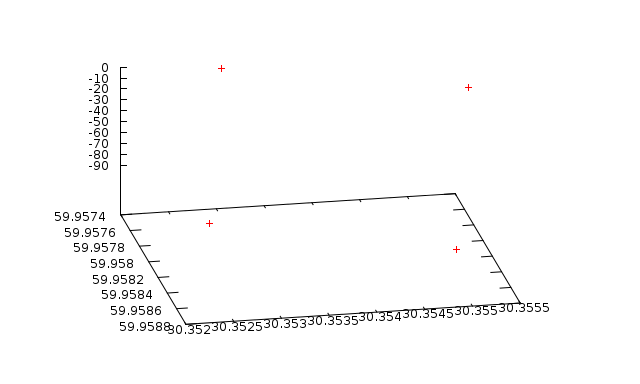
\includegraphics[width=\linewidth]{squaretopology.png}
    \caption{Topologia a 4 nodi}
    \label{fig:my_label}
\end{figure}
Questa e' la topologia di maggior interesse visto che, dato il costo del dispiegamento di sensori fissi dotati di modem acustico, si tende a ridurre al minimo il numero stesso di questi nodi.

\subsubsection{Topologia 6 nodi}
Nella topologia a 6 nodi, i nodi fissi sono disposti ai vertici di quello che, visto dall'alto, risulta essere un esagono. Tutti i nodi sono ad altezze diverse fra loro.   
\begin{figure}[H]
    \centering
    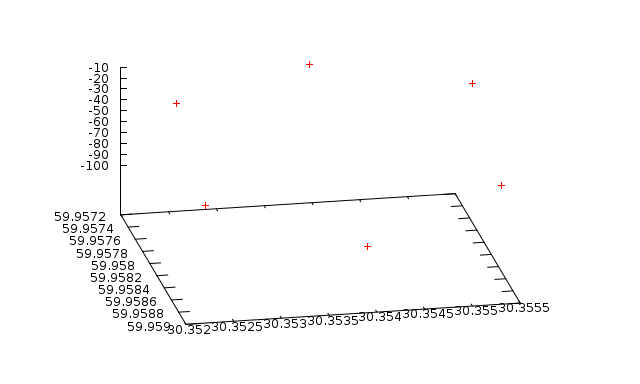
\includegraphics[width=\linewidth]{topologyhexagon.png}
    \caption{Topologia a 6 nodi}
    \label{fig:my_label}
\end{figure}
\subsubsection{Topologia 8 nodi}
Nella topologia a 8 nodi, i nodi fissi sono disposti ai vertici di un ottagono, a diverse altezze.
\begin{figure}[H]
    \centering
    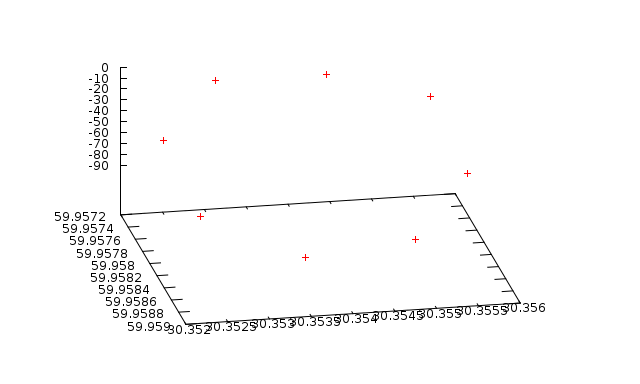
\includegraphics[width=\linewidth]{topologyoctagon.png}
    \caption{Topologia a 8 nodi}
    \label{fig:my_label}
\end{figure}

\section{Risultati della simulazione}
In questa sezione vengono riportati i risultati delle simulazioni svolte per le diverse topologie di rete sopra discusse. In ciascun grafico verranno riportati gli andamenti delle misurazioni impostando la soglia del valore di condizionamento rispettivamente ai valori 4, 7 e 10 (gli estremi del range simulativo ed il valore mediano).  
\subsection{Topologia a 4 nodi}
In primis, riportiamo i grafici per quanto concerne la situazione di AUV fermo nel punto "centrale" della topologia (proiettando i punti su piano x-y). Questa configurazione serve a simulare la modalita' operativa in cui, prima di effettuare la localizzazione, si obbliga il veicolo mobile a fermarsi. Se cio' puo' comportare una perdita di tempo rispetto alla missione cui e' assegnato l'AUV, di contro sia l'accuratezza che la precisione della localizzazione ottenuta sono elevate.

\begin{figure}[H]
    \centering
    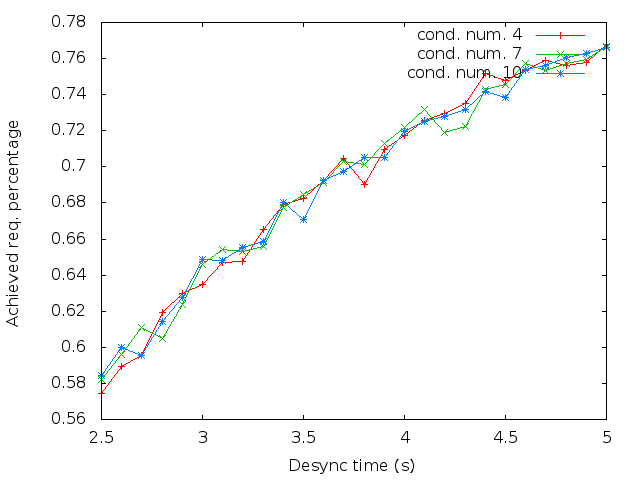
\includegraphics[scale=0.5]{squaresimulation/achievedlocpreempt0drop0speed0.png}
    \caption{Localizzazioni andate a buon fine}
    \label{fig:squaresimulation/achievedlocpreempt0drop0speed0}
\end{figure}

Il grafico ci anticipa, come si osservera' nel resto della sezione dedicata a questa topologia, l'irrilevanza della soglia del numero di condizionamento. Difatti trovandosi le proiezioni sul piano orizzontale delle posizioni dei nodi fissi ai vertici di un quadrato, l'allineamento fra queste posizioni e' minimo e di conseguenza anche il valore del numero di condizionamento sara' basso. Aumentando il valore del timer di desincronizzazione delle risposte, aumenta la percentuale di localizzazioni andate a buon fine, come ci si aspetta. E' da considerare, com'anche nelle successive simulazioni, che l'AUV si trova fermo in posizione quasi equidistante dai nodi fissi, da cui la necessita' di aumentare di molto il valore del tempo di desincronizzazione per evitare collisioni. Le stesse richieste effettuate in una posizione piu' decentrata avrebbero sicuramente necessitato di un minor valore del timer per ottenere pari risultati in termini di successo della localizzazione.
Per quanto riguarda l'errore medio e l'errore massimo sulla posizione calcolata, esso e' praticamente nullo, essendo entrambi minori di 10 $cm$.
In questa particolare situazione, variare modalita' di funzionamento del protocollo o soglia minima di richieste necessarie non causa praticamente mutazioni nei risultati ottenuti.

\begin{figure}[H]
    \centering
    \subfloat[Errore medio]{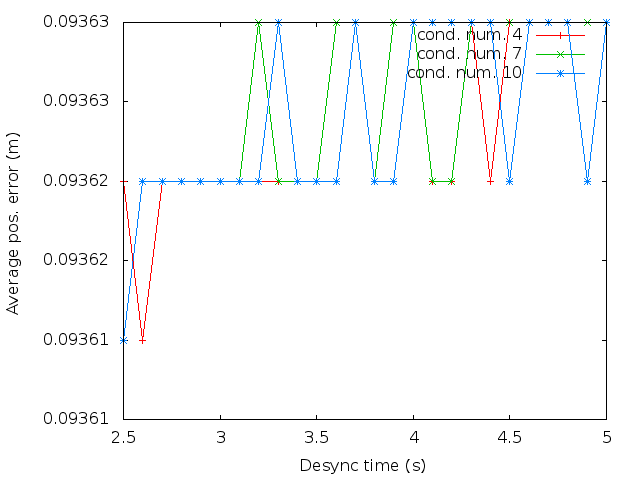
\includegraphics[width=0.4\textwidth]{squaresimulation/avposerrorpreempt0drop0speed0.png}
    \label{fig:squaresimulation/avposerrorpreempt0drop0speed0.png}}
    \hfill
    \subfloat[Errore massimo]{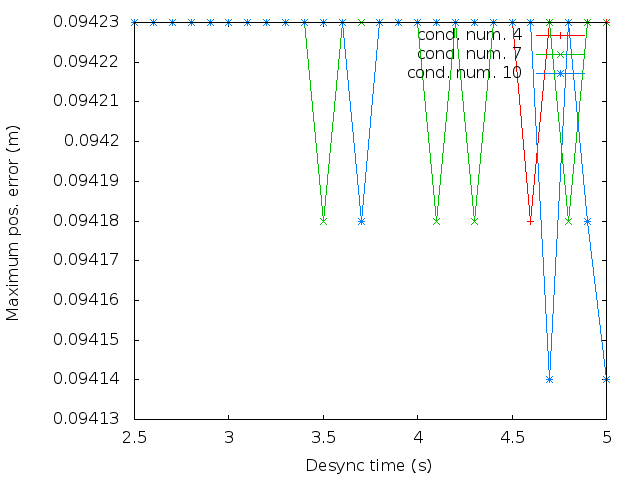
\includegraphics[width=0.4\textwidth]{squaresimulation/maxposerrorpreempt0drop0speed0.png}
    \label{fig:squaresimulation/maxposerrorpreempt0drop0speed0}}
\end{figure}

Di maggiore interesse sono i risultati ottenuti facendo muovere l'AUV a velocita' di 1 $\frac{m}{s}$. Riportiamo subito i grafici, confrontando la configurazione in cui si richiedono tre riposte con quella in cui ne richiediamo quattro.

\begin{figure}[H]
    \centering
    \subfloat[3 richieste]{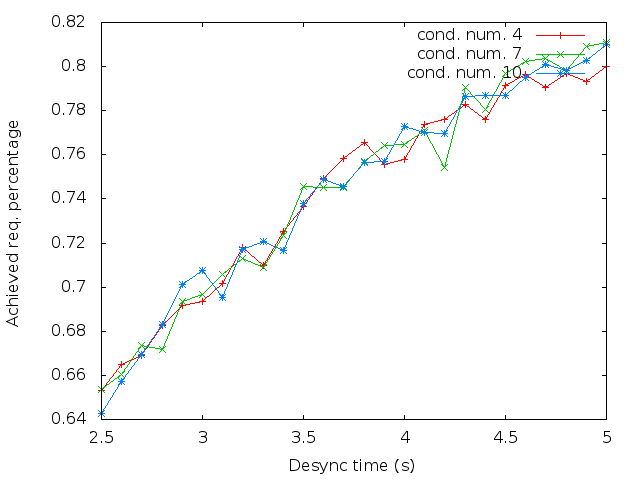
\includegraphics[width=0.4\textwidth]{squaresimulation/achievedlocreq3preempt0drop0speed1.png}
    \label{fig:squaresimulation/achievedlocreq3preempt0drop0speed1}}
    \hfill
    \subfloat[4 richieste]{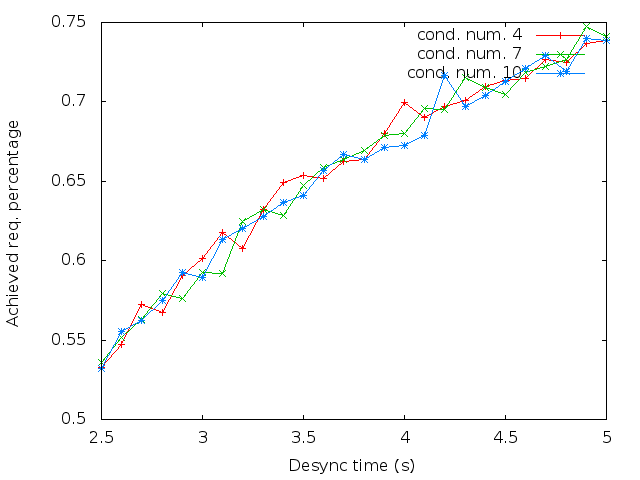
\includegraphics[width=0.4\textwidth]{squaresimulation/achievedlocreq4preempt0drop0speed1.png}
    \label{fig:squaresimulation/achievedlocreq3preempt0drop0speed1}}
    \caption{Percentuale di richieste portate a termine}
\end{figure}

\begin{figure}[H]
    \centering
    \subfloat[3 richieste]{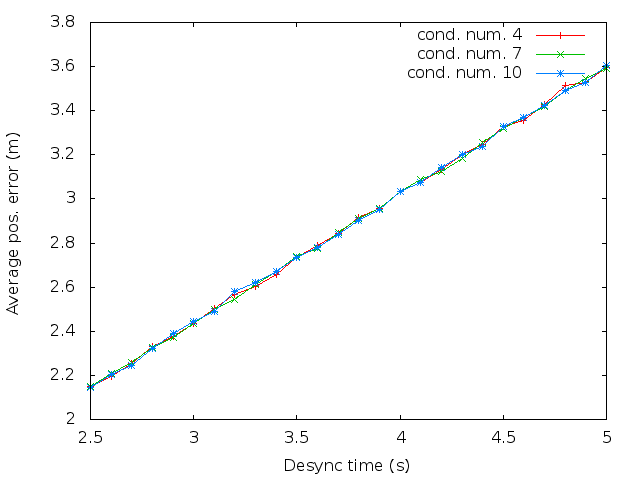
\includegraphics[width=0.4\textwidth]{squaresimulation/avposerrorreq3preempt0drop0speed1.png}
    \label{fig:squaresimulation/avposerrorreq3preempt0drop0speed1}}
    \hfill
    \subfloat[4 richieste]{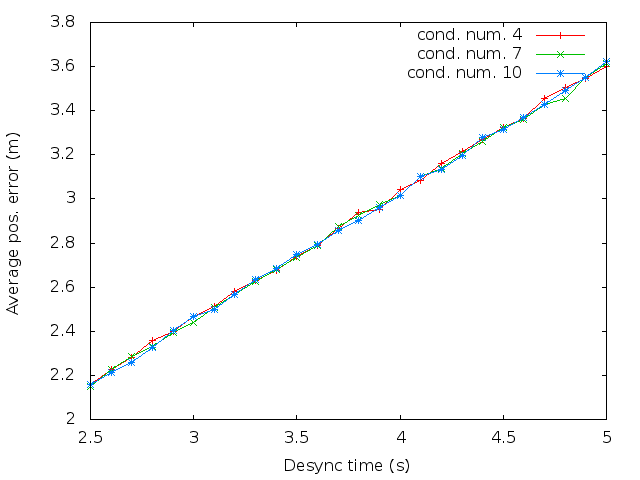
\includegraphics[width=0.4\textwidth]{squaresimulation/avposerrorreq4preempt0drop0speed1.png}
    \label{fig:squaresimulation/avposerrorreq4preempt0drop0speed1}}
    \caption{Errore medio}
\end{figure}

\begin{figure}[H]
    \centering
    \subfloat[3 richieste]{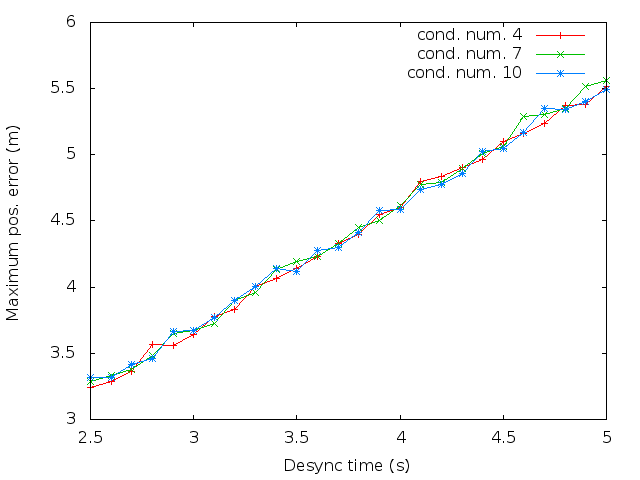
\includegraphics[width=0.4\textwidth]{squaresimulation/maxposerrorreq3preempt0drop0speed1.png}
    \label{fig:squaresimulation/maxposerrorreq3preempt0drop0speed1}}
    \hfill
    \subfloat[4 richieste]{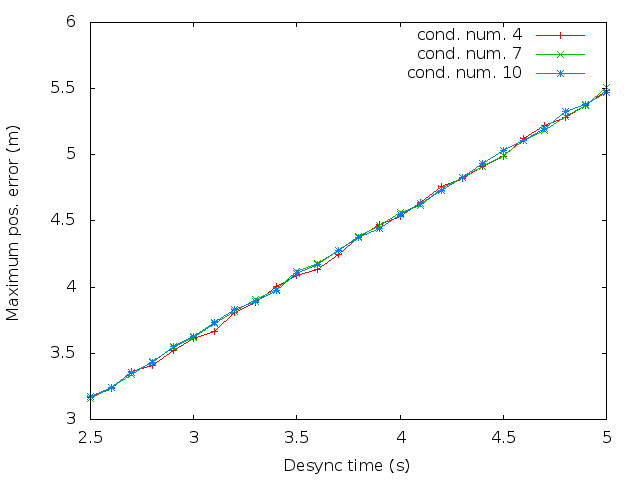
\includegraphics[width=0.4\textwidth]{squaresimulation/maxposerrorreq4preempt0drop0speed1.png}
    \label{fig:squaresimulation/maxposerrorreq4preempt0drop0speed1}}
    \caption{Errore massimo}
\end{figure}

In primis, si evince come l'attesa di una risposta in piu' rispetto al numero minimo di 3 non sortisca effetti positivi degni di nota. Al contrario, causa la diminuzione della percentuale di localizzazioni riuscite (di circa il 5 per tempo di desincronizzazione pari a 4.5 $s$\%).
Ci limitiamo quindi all'analisi della simulazione fatta attendendo 3 risposte.
Potendo considerare come sufficiente una percentuale di localizzazioni riuscite pari al 70\%, questo risultato viene raggiunto con un tempo di desincronizzazione di poco piu' di 3 secondi. Per questo valore, l'errore medio risulta essere di circa 2.5 $m$ mentre l'errore massimo e' di circa 3.7 $m$.
Col valore massimo considerato per il timer (5 $s$), questi due valori salgono a 3.6 e 5.5 $m$ rispettivamente, con un guadagno sulle localizzazioni positivamente effettutate di circa un 10\%.

E' stato interessante a questo punto verificare se la modalita' "preemptive" potesse in qualche modo migliorare i risultati fin qui ottenuti.
Se l'andamento della percentuale delle localizzazioni riuscite non viene modificato, si ottiene altresi' un notevole miglioramento delle prestazioni per quanto riguarda l'errore nel calcolo delle coordinate dell'AUV.

\begin{figure}
    \centering
    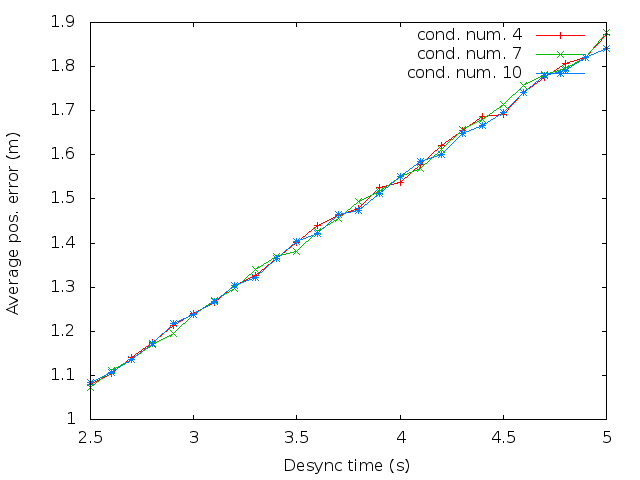
\includegraphics[scale=0.5]{squaresimulation/avposerrorreq3preempt1drop0speed1.png}
    \caption{Errore medio}
    \label{fig:squaresimulation/avposerrorreq3preempt1drop0speed1}
\end{figure}

\begin{figure}
    \centering
    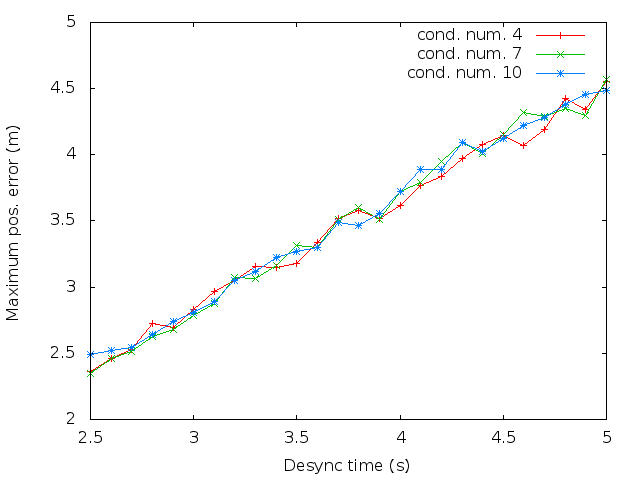
\includegraphics[scale=0.5]{squaresimulation/maxposerrorreq3preempt1drop0speed1.png}
    \caption{Errore massimo}
    \label{fig:squaresimulation/maxposerrorreq3preempt1drop0speed1}
\end{figure}

Il miglioramento rispetto alla modalita' normale e' evidente. Considerando di nuovo la soglia del 70\% di localizzazioni riuscite, in corrispondenza di quel valore abbiamo un errore medio sulle coordinate calcolate del veicolo di circa 1.25 $m$ ed un errore massimo di circa 2.8 $m$. Prendendo il massimo valore del timer di desincronizzazione, l'errore medio comunque non sale oltre i 2 $m$, meno della meta' del valore in ~\ref{fig:squaresimulation/maxposerrorreq3preempt0drop0speed1}.
Come ci si aspettava, il movimento dell'AUV durante l'attesa dello scadere del timer per effettuare il calcolo della posizione e' uno dei fattori che piu' influenzano negativamente la precisione della localizzazione. La modalita' "preemptive", che ne diminuisce l'effetto, genera quindi un netto miglioramento nelle prestazioni del protocollo.
Riportiamo ora i risultati considerando un AUV che si stia movendo al doppio della velocita' or ora considerata, ovverro 2 $\frac{m}{s}$.
Di nuovo, la configurazione in cui si richiedono un minimo di 4 risposte non genera' risultati diversi dalla versione a 3 risposte.
Confrontiamo i risultati in modalita' preemptive e non preemptive, per evidenziare ulteriormente la bonta' di tale modalita'.

\begin{figure}[H]
    \centering
    \subfloat[Non Preemptive]{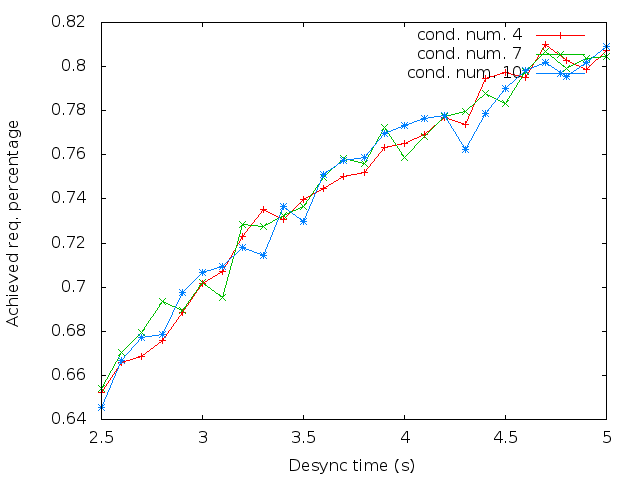
\includegraphics[width=0.4\textwidth]{squaresimulation/achievedlocreq3preempt0drop0speed2.png}
    \label{fig:squaresimulation/achievedlocreq3preempt0drop0speed2}}
    \hfill
    \subfloat[Preemptive]{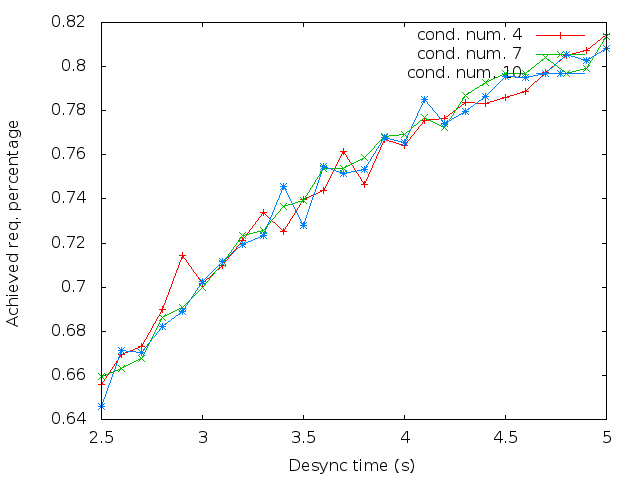
\includegraphics[width=0.4\textwidth]{squaresimulation/achievedlocreq3preempt1drop0speed2.png}
    \label{fig:squaresimulation/achievedlocreq3preempt1drop0speed2}}
    \caption{Localizzazioni riuscite}
\end{figure}

\begin{figure}[H]
    \centering
    \subfloat[Non Preemptive]{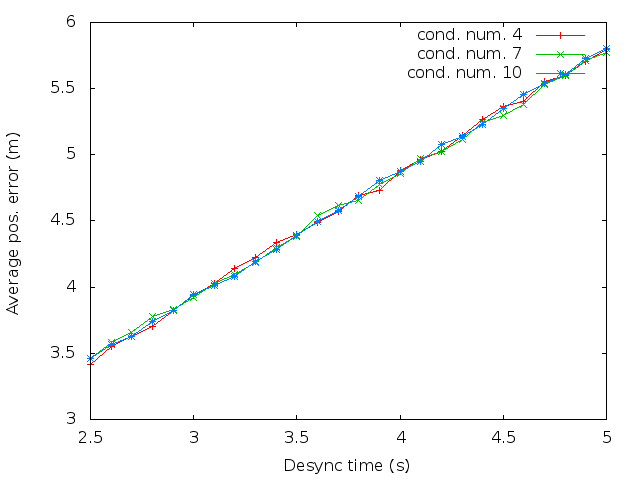
\includegraphics[width=0.4\textwidth]{squaresimulation/avposerrorreq3preempt0drop0speed2.png}
    \label{fig:squaresimulation/avposerrorreq3preempt0drop0speed2}}
    \hfill
    \subfloat[Preemptive]{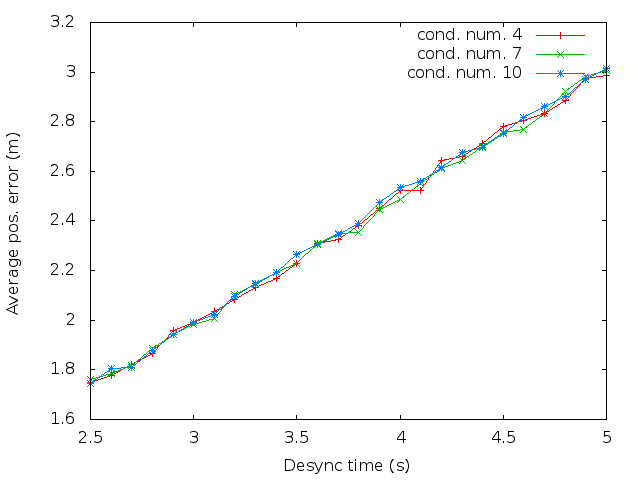
\includegraphics[width=0.4\textwidth]{squaresimulation/avposerrorreq3preempt1drop0speed2.png}
    \label{fig:squaresimulation/avposerrorreq3preempt1drop0speed2}}
    \caption{Errore medio}
\end{figure}

\begin{figure}[H]
    \centering
    \subfloat[Non Preemptive]{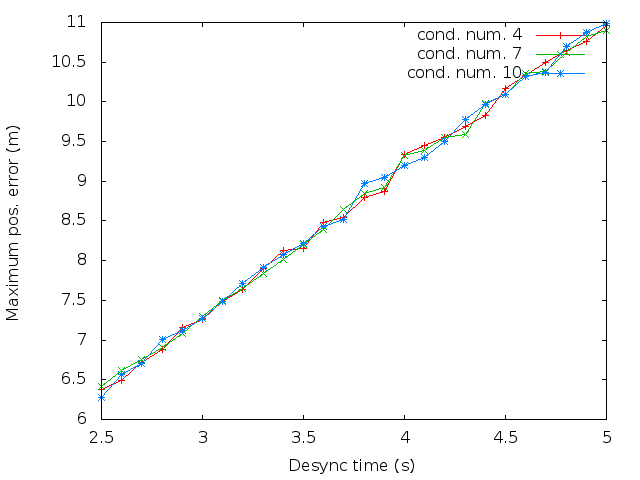
\includegraphics[width=0.4\textwidth]{squaresimulation/maxposerrorreq3preempt0drop0speed2.png}
    \label{fig:squaresimulation/maxposerrorreq3preempt0drop0speed2}}
    \hfill
    \subfloat[Preemptive]{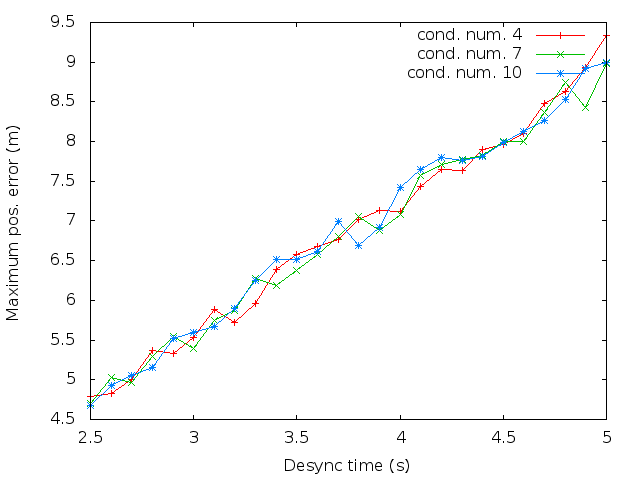
\includegraphics[width=0.4\textwidth]{squaresimulation/maxposerrorreq3preempt1drop0speed2.png}
    \label{fig:squaresimulation/maxposerrorreq3preempt1drop0speed2}}
    \caption{Errore massimo}
\end{figure}
Anche alla velocita' di punta di 2 $\frac{m}{s}$, si potrebbe garantire, con probabilita' di riuscita della localizzazione del 70\%, un errore sulla posizione di circa 2 $m$ ed errore massimo di 5.5 $m$, valori non da sottovalutare dato che si tratta di una velocita' abbastanza elevata per questo tipo di dispositivi. 

\subsection{Topologia a 6 nodi}
Passiamo ora in rassegna i risultati ottenuti con la topologia a 6 nodi fissi.
Nelle simulazioni ci si aspettava che l'aggiunta di due nodi fissi avrebbe migliorato, se non l'errore della posizione calcolata rispetto alla posizione reale, almeno la percentuale di localizzazioni andata a buon fine, essendoci due nodi in piu' da cui l'AUV potesse ricevere risposta. Effettivamente, imponendo la soglia minima di risposte pari a 3 e AUV fermo, rispetto alla configurazione a 4 nodi fissi c'e' un netto aumento della percentuale delle richieste di localizzazione riuscite:
\begin{figure}[H]
    \centering
    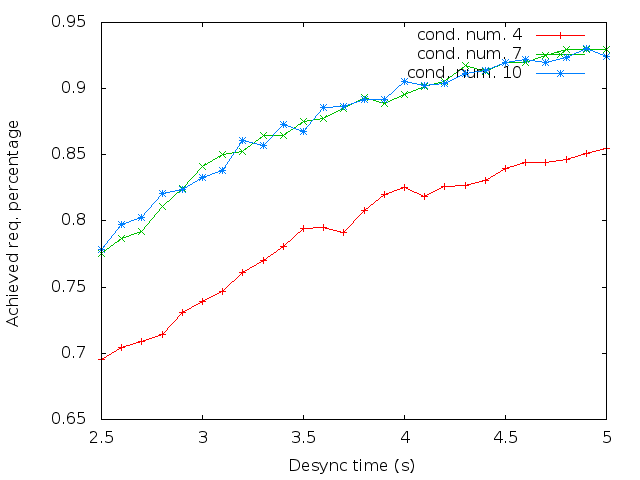
\includegraphics[scale=0.5]{hexagonsimulation/achievedlocreq3preempt0drop0speed0.png}
    \caption{Percentuale localizzazioni riuscite}
    \label{fig:hexagonsimulation/achievedlocreq3preempt0drop0speed0}
\end{figure}
La media dell'errore sulla posizione calcolata, come in ~\ref{fig:squaresimulation/avposerrorpreempt0drop0speed0.png}, e' all'incirca di 10 $cm$, mentre l'errore massimo misurato e' di circa 20 $cm$ con numero di condizionamento massimo uguale a 4 mentre risulta essere di circa 30 $cm$ negli altri due casi.
Rispetto alla topologia a 4 nodi, notiamo come in questa situazione il valore utilizzato come soglia per il numero di condizionamento influenzi in maniera decisiva il funzionamento del protocollo. Difatti, nella topologia a 6 nodi fissi, e' probabile che in alcuni casi l'AUV riceva risposte da nodi fra loro vicini ed allineati (l'angolo fra 3 nodi consecutivi di un esagono e' di 120 gradi, mentre per il quandrato sono 90 gradi). Di qui l'aumento del valore medio del numero di condizionamento, che in certi casi si trova la soglia impostata. A questo fenomeno abbiamo ricondotto la differenza fra il grafico con soglia pari a 4 e quello con soglia pari a 7 e 10, dove invece le richieste non andate a buon fine sono quasi tutte da imputare a collisioni fra le risposte inviate dai nodi fissi.
Si e' cercata quindi una soluzione che garantisse la maggior precisione di una soglia bassa per il numero di condizionamento combinando al tempo stesso la percentuale di localizzazioni riuscite.
Da qui nasce la modalita' "droponepoint", che da' all'AUV la possibilita' di scartare iterativamente una delle risposte ricevute e ripetere il calcolo della propria posizione, sperando di rientrare all'interno della soglia prestabilita per il numero di condizionamento. Riportiamo il grafico del funzionamento del protocollo nella situazione analoga a quella presentata nel grafico precedente, ma con la modalita' "droponepoint" attivata:
\begin{figure}[H]
    \centering
    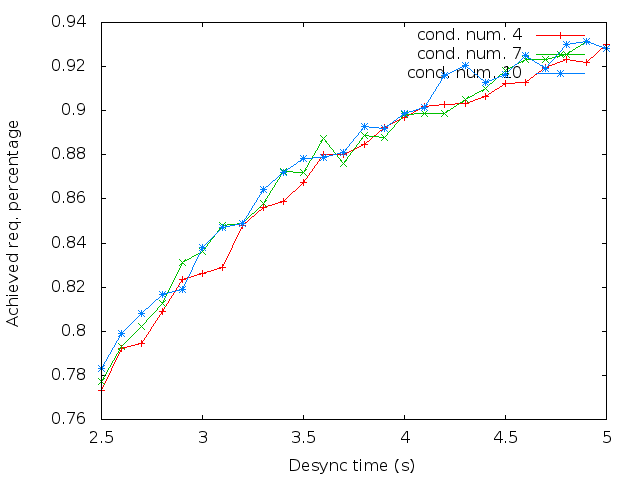
\includegraphics[scale=0.5]{hexagonsimulation/achievedlocreq3preempt0drop1speed0.png}
    \caption{Percentuale localizzazioni riuscite}
    \label{fig:hexagonsimulation/achievedlocreq3preempt0drop1speed0}
\end{figure}
Con la modalita' attivata, la percentuale di localizzazioni successful per valore soglia pari a 4 raggiunge quella degli altri due grafici, mantenendo inalterati i valori dell'errore medio e dell'errore massimo. 
Come per la topologia a 4 nodi, aumentare la soglia minima di richieste con il veicolo fermo non migliora l'efficienza del protocollo. Al contrario, la percentuale di localizzazioni andate a buon fine diminuisce di molto, mentre l'errore medio e' piu' o meno uguale. Migliora solamente l'errore massimo (diviene anch'esso di poco superiore ai 10 $cm$), in conformita' col comportamento previsto dal metodo matematico utilizzato per calcolare le coordinate dell'AUV (un maggior numero di risposte implica un numero di condizionamento minore e dunque una minor propagazione dell'errore sulle distanza nel calcolo della posizione).
Consideriamo ora le situazioni in cui imposto la soglia minima di risposte rispettivamente a 3 e 4, facendo muovere l'AUV ad 1 $\frac{m}{s}$.
Riportiamo direttamente i grafici ottenuti attivando la modalita' "preemptive". Confrontiamo i risultati ottenuti utilizzando solamente questa modalita' e quelli ottenuti in combinazione con la modalita' "droponepoint", attivata per la configurazione con soglia minima di risposte impostata a 4.


\begin{figure}[H]
    \centering
    \subfloat[Non Droponepoint]{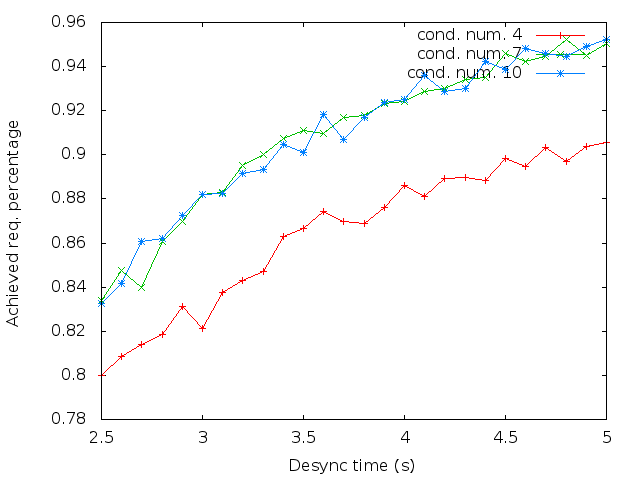
\includegraphics[width=0.4\textwidth]{hexagonsimulation/achievedlocreq3preempt1drop0speed1.png}
    \label{fig:hexagonsimulation/achievedlocreq3preempt1drop0speed1}}
    \hfill
    \subfloat[Droponepoint]{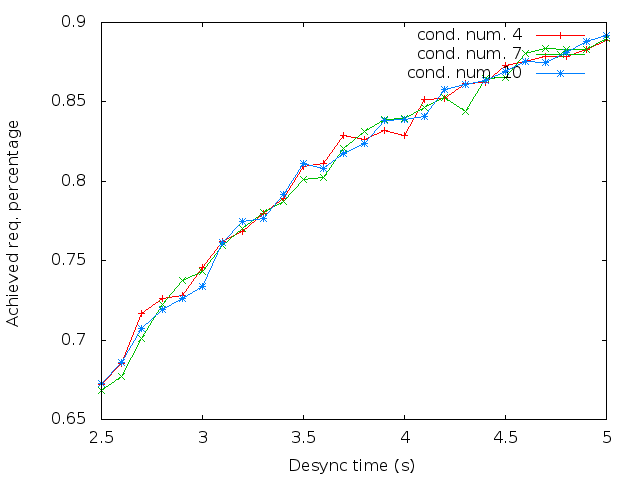
\includegraphics[width=0.4\textwidth]{hexagonsimulation/achievedlocreq4preempt1drop1speed1.png}
    \label{fig:hexagonsimulation/achievedlocreq4preempt1drop1speed1}}
    \caption{Localizzazioni riuscite}
\end{figure}

\begin{figure}[H]
    \centering
    \subfloat[Non Droponepoint]{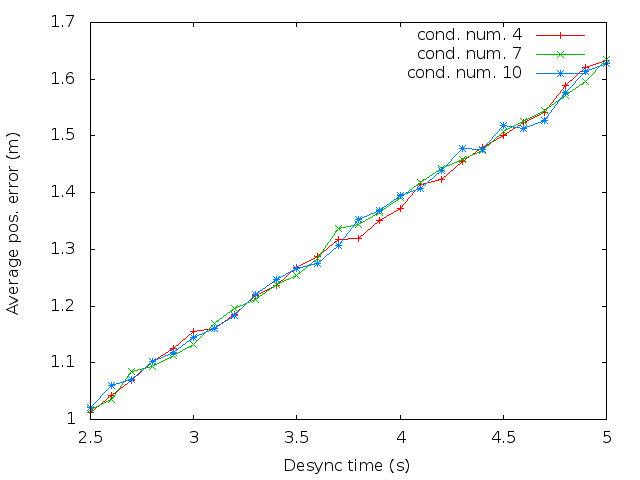
\includegraphics[width=0.4\textwidth]{hexagonsimulation/avposerrorreq3preempt1drop0speed1.png}
    \label{fig:hexagonsimulation/avposerrorreq3preempt1drop0speed1}}
    \hfill
    \subfloat[Droponepoint]{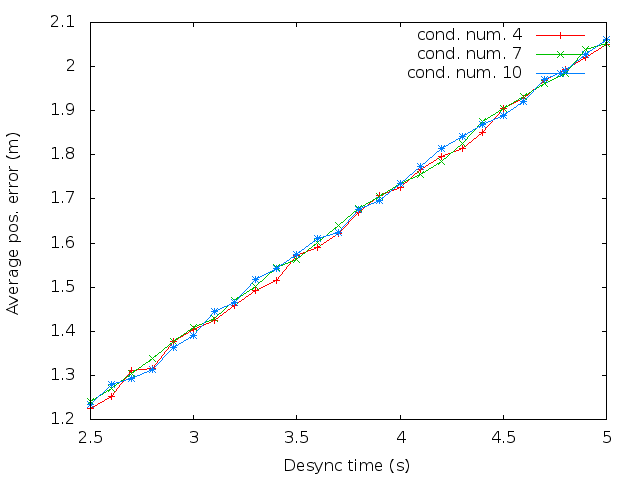
\includegraphics[width=0.4\textwidth]{hexagonsimulation/avposerrorreq4preempt1drop1speed1.png}
    \label{fig:hexagonsimulation/avposerrorreq4preempt1drop1speed1.png}}
    \caption{Errore medio}
\end{figure}

\begin{figure}[H]
    \centering
    \subfloat[Non Droponepoint]{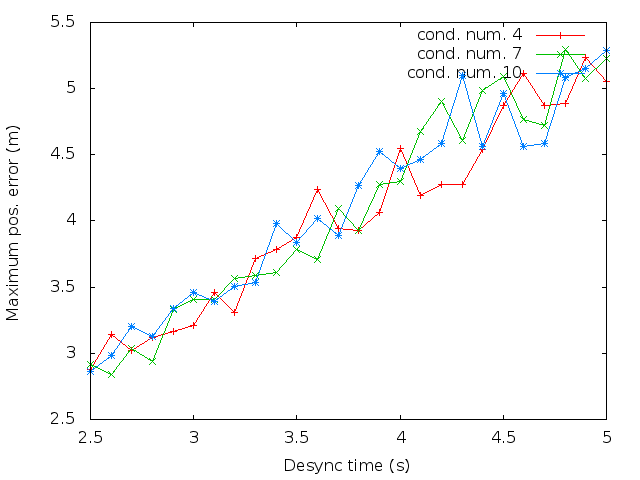
\includegraphics[width=0.4\textwidth]{hexagonsimulation/maxposerrorreq3preempt1drop0speed1.png}
    \label{fig:hexagonsimulation/maxposerrorreq3preempt1drop0speed1}}
    \hfill
    \subfloat[Droponepoint]{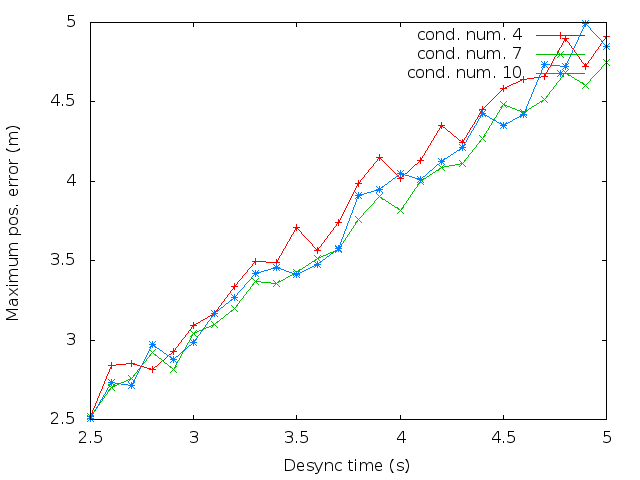
\includegraphics[width=0.4\textwidth]{hexagonsimulation/maxposerrorreq4preempt1drop1speed1.png}
    \label{fig:hexagonsimulation/maxposerrorreq4preempt1drop1speed1}}
    \caption{Errore massimo}
\end{figure}
La soglia impostata a 3 risposte fa si che la percentuale di richieste di localizzazione riuscite con questo valore sia piu' alto, almeno per quanto riguarda i grafici per numero di condizionamento 7 e 10, rispetto alla percentuale per la soglia impostata a 4 risposte (quest'ultima percentuale e', tra l'altro, incrementata dalla modalita' "droponepoint").
Nel confronto degli errori le due configurazioni mostrano profonde differenze. In primis, configurazione "preemptive"-3 risposte riesce ad ottenere un 80\% e piu' di localizzazioni riuscite con un tempo di desincronizzazione minino di 2.5 $s$, al contrario dei circa 3.5 $s$ necessari all'altra configurazione. Per questi valori, i grafici a sinistra riportano un errore medio di circa 1 $m$ (con errore massimo di poco meno di 3 $m$), mentre la modalita' "droponepoint" genera un errore medio di circa 1.5 $m$ ed errore massimo di 3.5 $m$.
Oltre ad ottenre un guadagno di precisione di circa 0.5 $m$, la configurazione mostrata nei grafici a sinistra arriva a questo risultato risparmiando all'incirca 1 $s$ nel timer di desincronizzazione dei nodi fissi (il che permette nel lungo periodo di effettuare richieste di localizzazione con piu' frequenza).
Riportiamo il confronto fra le stesse identiche configurazioni, portando la velocita' a 2 $\frac{m}{s}$.

\begin{figure}[H]
    \centering
    \subfloat[Non Droponepoint]{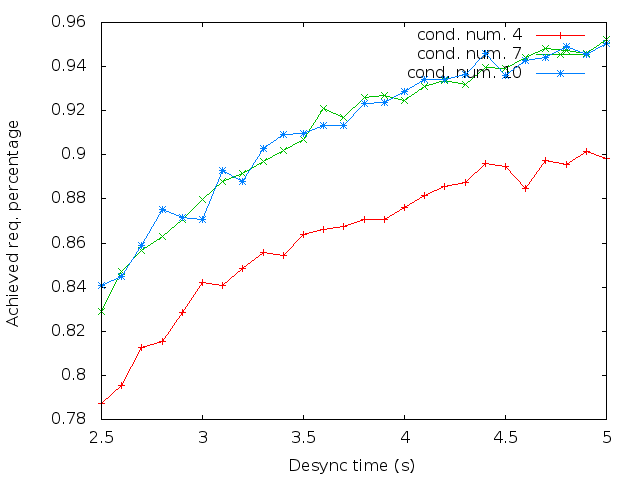
\includegraphics[width=0.4\textwidth]{hexagonsimulation/achievedlocreq3preempt1drop0speed2.png}
    \label{fig:hexagonsimulation/achievedlocreq3preempt1drop0speed2}}
    \hfill
    \subfloat[Droponepoint]{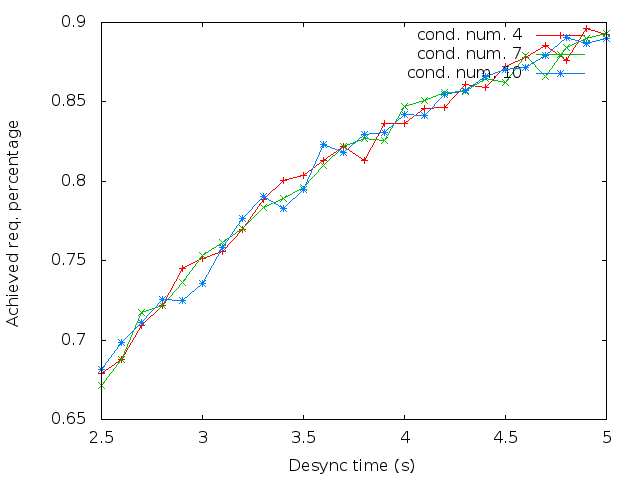
\includegraphics[width=0.4\textwidth]{hexagonsimulation/achievedlocreq4preempt1drop1speed2.png}
    \label{fig:hexagonsimulation/achievedlocreq4preempt1drop1speed2}}
    \caption{Localizzazioni riuscite}
\end{figure}

\begin{figure}[H]
    \centering
    \subfloat[Non Droponepoint]{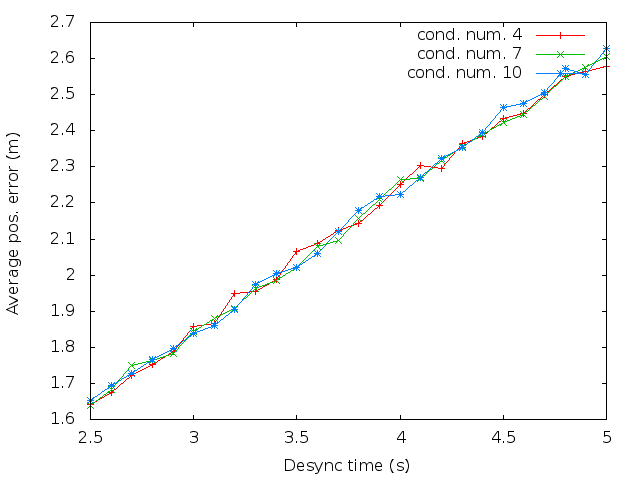
\includegraphics[width=0.4\textwidth]{hexagonsimulation/avposerrorreq3preempt1drop0speed2.png}
    \label{fig:hexagonsimulation/avposerrorreq3preempt1drop0speed2}}
    \hfill
    \subfloat[Droponepoint]{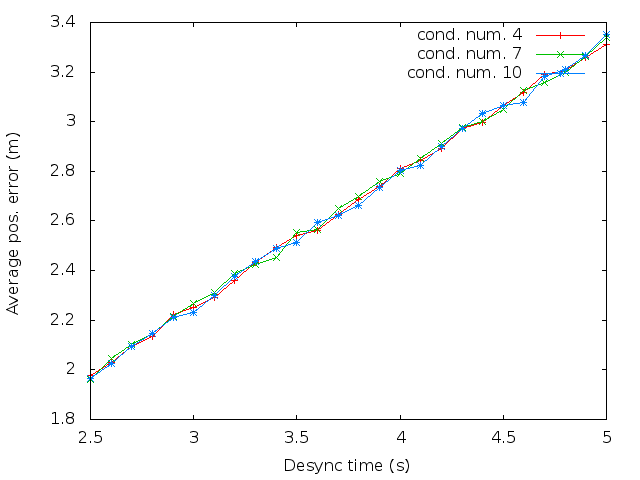
\includegraphics[width=0.4\textwidth]{hexagonsimulation/avposerrorreq4preempt1drop1speed2.png}
    \label{fig:hexagonsimulation/avposerrorreq4preempt1drop1speed2.png}}
    \caption{Errore medio}
\end{figure}

\begin{figure}[H]
    \centering
    \subfloat[Non Droponepoint]{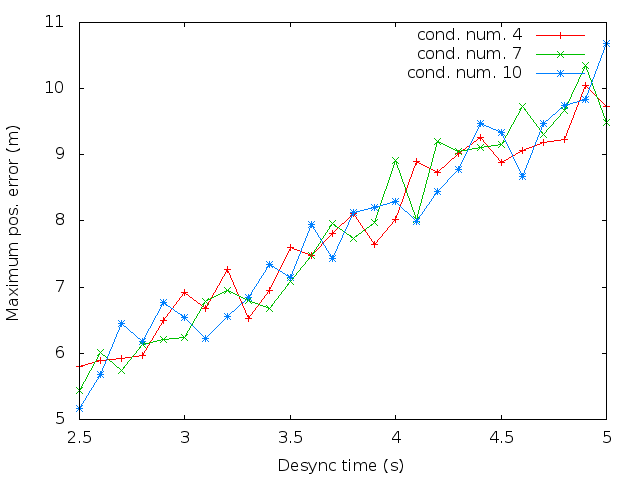
\includegraphics[width=0.4\textwidth]{hexagonsimulation/maxposerrorreq3preempt1drop0speed2.png}
    \label{fig:hexagonsimulation/maxposerrorreq3preempt1drop0speed2}}
    \hfill
    \subfloat[Droponepoint]{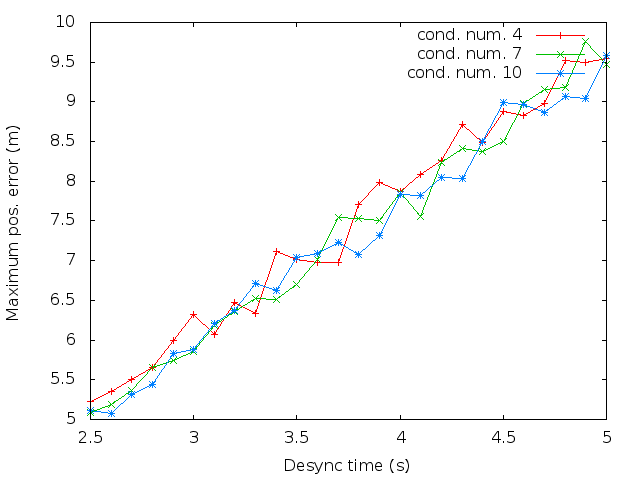
\includegraphics[width=0.4\textwidth]{hexagonsimulation/maxposerrorreq4preempt1drop1speed2.png}
    \label{fig:hexagonsimulation/maxposerrorreq4preempt1drop1speed2}}
    \caption{Errore massimo}
\end{figure}

Come si nota, modificando la velocita', non mutano le caratteristiche e le differenze fra le due configurazioni. Di nuovo, la configurazione con soglia minima di risposte impostata a 3 e modalita' "preemptive" attivata risulta vincente.

\subsection{Topologia a 8 nodi}
In ultimo, riportiamo i risultati per la topologia di rete comprendente 8 nodi fissi. 
Come per le altre topologie, presentiamo inizialmente la configurazione con AUV fermo al "centro" della costellazione dei nodi fissi. La soglia minima di risposte richiesta e' pari a 3 e ne' la modalita' "preemptive" ne' quella "droponepoint" sono attivate:
\begin{figure}[H]
    \centering
    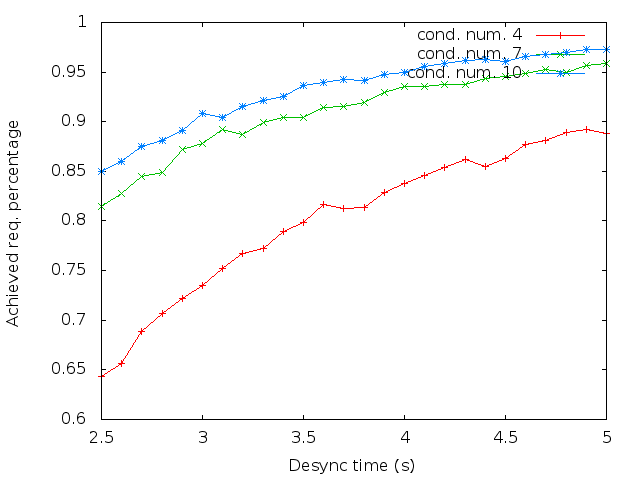
\includegraphics[scale=0.5]{octagonsimulation/achievedlocreq3preempt0drop0speed0.png}
    \caption{Percentuale localizzazioni riuscite}
    \label{fig:octagonsimulation/achievedlocreq3preempt0drop0speed0}
\end{figure}
\begin{figure}[H]
    \centering
    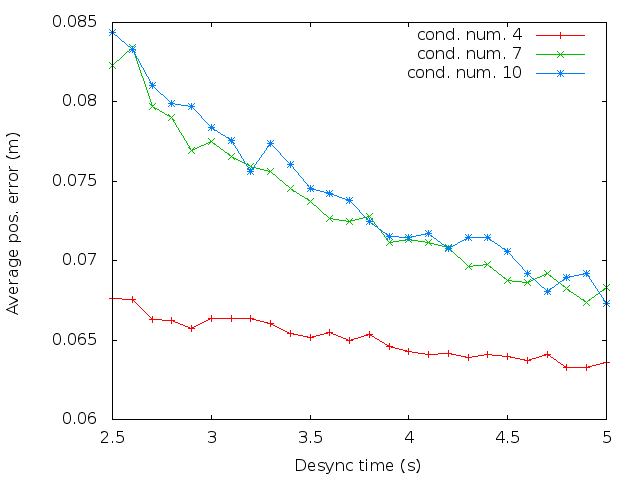
\includegraphics[scale=0.5]{octagonsimulation/avposerrorreq3preempt0drop0speed0.png}
    \caption{Errore medio}
    \label{fig:octagonsimulation/avposerrorreq3preempt0drop0speed0}
\end{figure}
\begin{figure}[H]
    \centering
    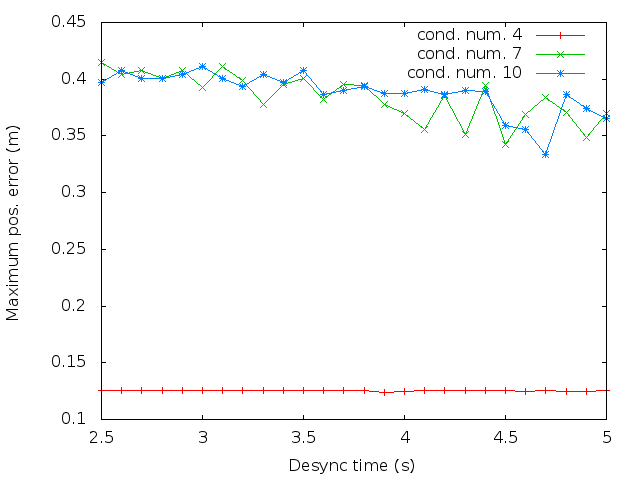
\includegraphics[scale=0.5]{octagonsimulation/maxposerrorreq3preempt0drop0speed0.png}
    \caption{Errore massimo}
    \label{fig:octagonsimulation/maxposerrorreq3preempt0drop0speed0}
\end{figure}
Come gia' evidenziato per la figura ~\ref{fig:hexagonsimulation/achievedlocreq3preempt0drop0speed0}(topologia a 6 nodi), risulta accentuata la differenza fra i grafici corrispondenti a valori-soglia diversi per il numero di condizionamento. In particolare, in figura \ref{fig:octagonsimulation/achievedlocreq3preempt0drop0speed0}, notiamo una differenziazione fra i grafici ottenuti rispettivamenti con numero di condizionamento massimo pari a 7 e 10. La topologia ad 8 nodi fa si che l'angolo massimo fra 3 nodi consecutivi sia di 135 gradi (rispetto ai 120 della topologia a 6 nodi), incrementando quindi il grado di collinearita' dei nodi, e dunque il valore medio del numero di condizionamento, di un'entita' tale da far si che anche stabilendo il valore 7 come massimo per il parametro in questione alcune richieste di localizzazione non vadano a buon fine a causa del superamento di tale soglia.
Tutti e tre i grafici concludono la loro curva (valore 5 $s$ del tempo massimo di desincronizzazione) a percentuali piu' elevate rispetto alle altre due topologie (l'aggiunta di altri 2 nodi fissi fa si che sia piu' probabile ricevere le 3 risposte che mi servono per effettuare la localizzazione). In particolare, e' notevole il fatto che  con numero di condizionamento pari a 10 si superi la percentuale del 97\% di successi, sfiorando la situazione ideale del 100\% di risultati positivi.
Per quanto riguarda l'errore medio, otteniamo dei valori estremamente precisi. Di piu' , rispetto alle altre topologie si denota un andamento decrescente dell'errore medio con l'aumentare del valore del timer di desincronizzazione, imputabile all'aumento di precisione del calcolo dovuto al maggior numero di risposte ricevute (ci aspetteremmo un andamento del genere ancora piu' marcato incrementando ulteriormente il numero di nodi fissi della rete).
L'errore massimo sul posizionamento e' molto ridotto per numero di condizionamento uguale a 4 (circa 12.5 $cm$), mentre negli altri due grafici si alza a circa 40 $cm$, mostrando un lieve andamento decrementale.
Aumentanre la soglia minima di risposte richieste non comporta un miglioramento netto delle prestazioni del protocollo, mentre diminuisce ovviamente la percentuale di localizzazioni riuscite.
Passiamo ora a considerare l'AUV in movimento (dapprima 1 $\frac{m}{s}$).
Confrontiamo i risultati ottenuti con soglia minima di risposte impostata a 3, utilizzando o meno la modalita' preemptive.
\begin{figure}[H]
    \centering
    \subfloat[Non Preemptive]{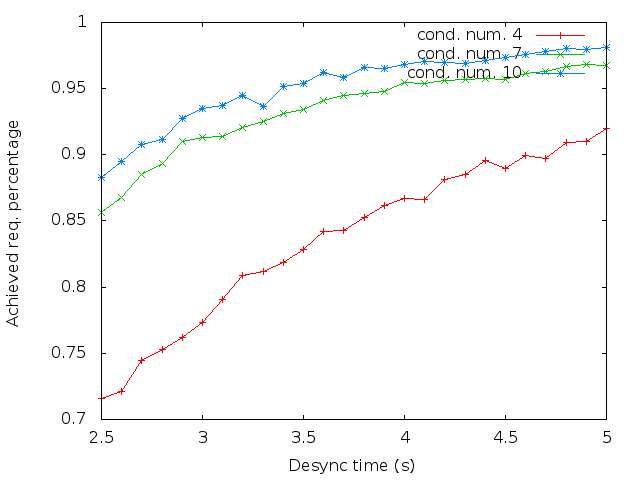
\includegraphics[width=0.4\textwidth]{octagonsimulation/achievedlocreq3preempt0drop0speed1.png}
    \label{fig:octagonsimulation/achievedlocreq3preempt0drop0speed1}}
    \hfill
    \subfloat[Preemptive]{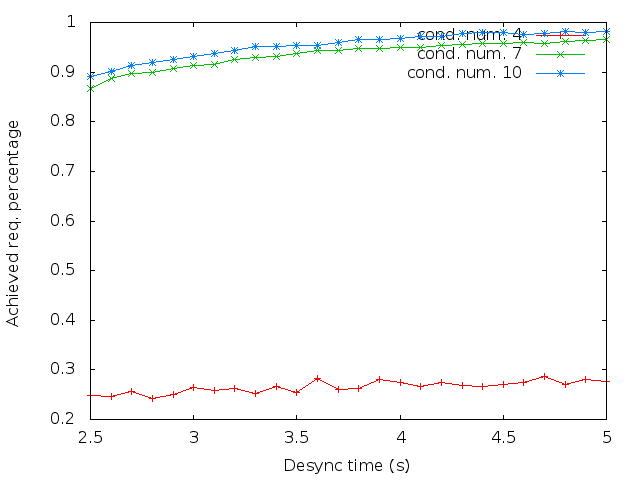
\includegraphics[width=0.4\textwidth]{octagonsimulation/achievedlocreq3preempt1drop0speed1.png}
    \label{fig:octagonsimulation/achievedlocreq3preempt1drop0speed1}}
    \caption{Localizzazioni riuscite}
\end{figure}

\begin{figure}[H]
    \centering
    \subfloat[Non Preemptive]{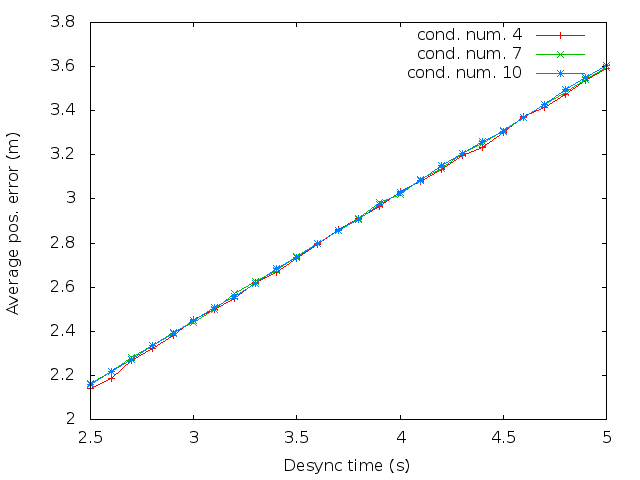
\includegraphics[width=0.4\textwidth]{octagonsimulation/avposerrorreq3preempt0drop0speed1.png}
    \label{fig:octagonsimulation/avposerrorreq3preempt0drop0speed1}}
    \hfill
    \subfloat[Preemptive]{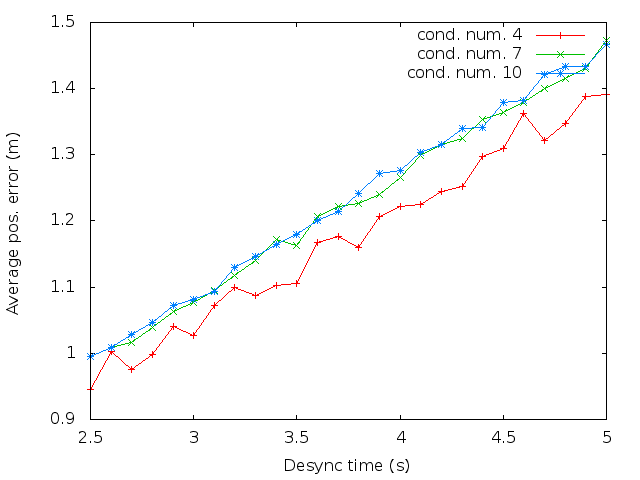
\includegraphics[width=0.4\textwidth]{octagonsimulation/avposerrorreq3preempt1drop0speed1.png}
    \label{fig:octagonsimulation/avposerrorreq3preempt1drop0speed1}}
    \caption{Errore medio}
\end{figure}

\begin{figure}[H]
    \centering
    \subfloat[Non Preemptive]{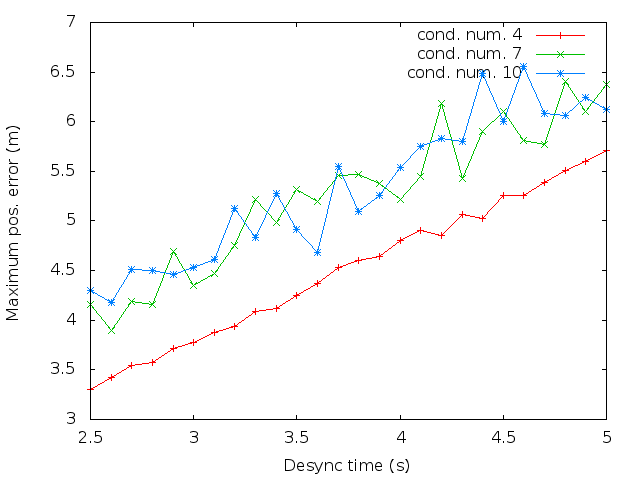
\includegraphics[width=0.4\textwidth]{octagonsimulation/maxposerrorreq3preempt0drop0speed1.png}
    \label{fig:octagonsimulation/maxposerrorreq3preempt0drop0speed1}}
    \hfill
    \subfloat[Preemptive]{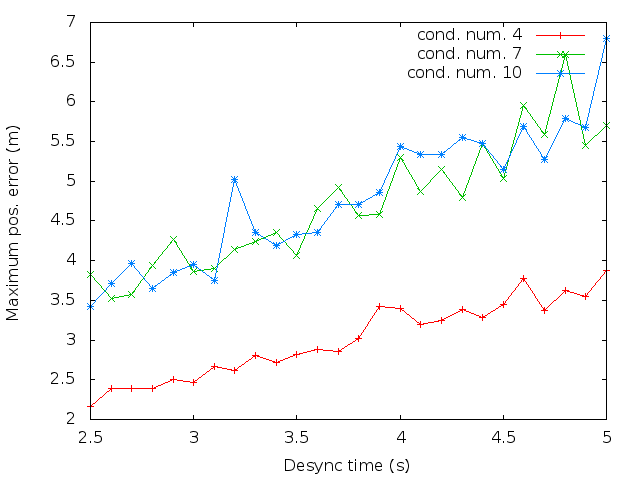
\includegraphics[width=0.4\textwidth]{octagonsimulation/maxposerrorreq3preempt1drop0speed1.png}
    \label{fig:octagonsimulation/maxposerrorreq3preempt1drop0speed1}}
    \caption{Errore massimo}
\end{figure}
Vediamo come fra la modalita' preemptive e quella normale vi sia una netta differenza per quanto riguarda il numero di localizzazioni andate a buon fine per quanto riguarda le simulazioni effettuate con soglia del numero di condizionamento pari a 4. La modalita' preemptive causa la drastica diminuzione delle localizzazioni riuscite (e' piu' probabile che le 3 risposte ricevute dall'AUV siano da nodi vicini tra loro e quindi abbastanza allineati), mentre la modalita' di funzionamento normale presenta dei valori simili alla configurazione con AUV fermo (\ref{fig:octagonsimulation/achievedlocreq3preempt0drop0speed0}).
In entrambe le configurazioni, nei grafici per i valori soglia del numero di condizionamento 7 o 10 le richieste di posizionamento riuscite partono da un valore superiore all'85\% , con tempo di desincronizzazione dei nodi fissi pari a 2.5 $s$.
Per questi valori, la modalita' preemptive genera un errore medio di circa 1 $m$ ed un errore massimo di 3.5 $m$. La modalita' di funzionamento normale invece effettua il calcolo delle coordinate dell'AUV con un errore medio di piu' di 2 $m$ ed un errore massimo di piu' di 4 $m$.
All'aumentare del tempo di desincronizzazione, il comportamento delle due modalita' differisce ulteriormente. L'errore medio della modalita' preemptive aumenta ma non in maniera decisiva, toccando il valore di quasi 1.5 $m$ per timer di desincronizzazione pari a 5 $s$, mentre l'errore medio nella modalita' normale sale a circa 3.5 $m$. Per la modalita' preemptive questo e' giustificato dal fatto che, pur aumentando il valore del timer, non appena il veicolo riceve 3 risposte effettua il calcolo della propria posizione. Essendoci 8 nodi fissi da cui poter ricevere risposta, cio' non avviene molto tempo dopo l'avvio del timer. Al contrario, nella modalita' normale l'aumento del tempo massimo di desincronizzazione causa l'effettiva dilatazione del tempo che intercorre tra l'arrivo delle risposte e l'avvio del calcolo delle coordinate (aumentando notevolmente l'errore del calcolo).
Riportiamo ora la configurazione in cui il nodo si muove sempre a velocita' di 1 $\frac{m}{s}$ , la soglia minima di risposte e' impostata a 4 nodi e sono attivate sia la modalita' "preemptive" che quella "droponepoint". 
\begin{figure}[H]
    \centering
    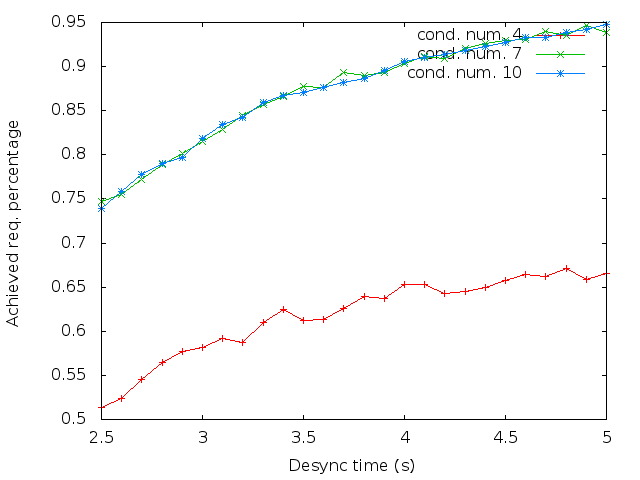
\includegraphics[scale=0.5]{octagonsimulation/achievedlocreq4preempt1drop1speed1.png}
    \caption{Percentuale localizzazioni riuscite}
    \label{fig:octagonsimulation/achievedlocreq4preempt1drop1speed1}
\end{figure}
\begin{figure}[H]
    \centering
    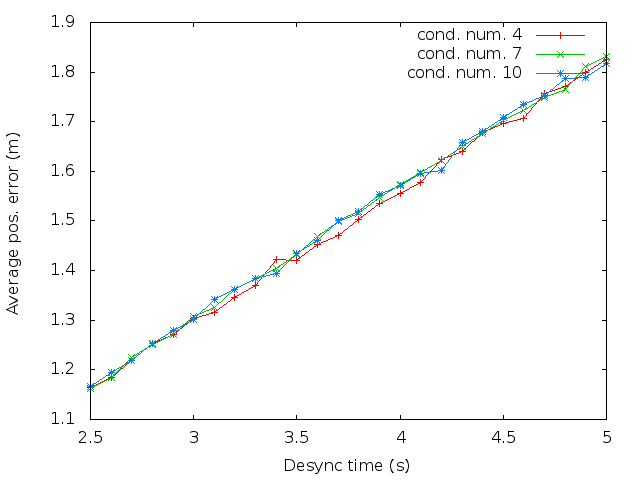
\includegraphics[scale=0.5]{octagonsimulation/avposerrorreq4preempt1drop1speed1.png}
    \caption{Errore medio}
    \label{fig:octagonsimulation/avposerrorreq4preempt1drop1speed1}
\end{figure}
\begin{figure}[H]
    \centering
    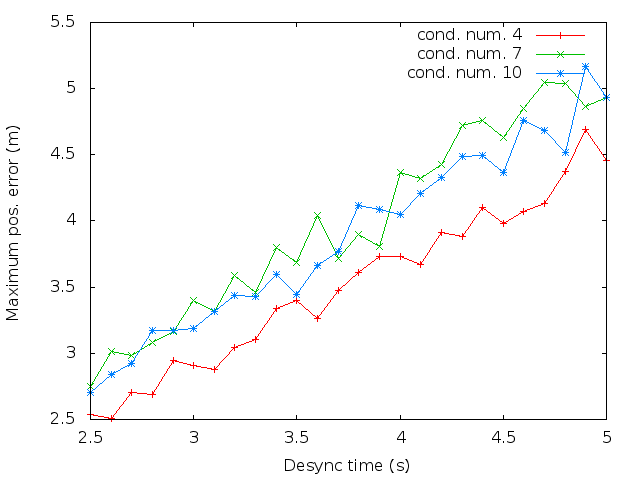
\includegraphics[scale=0.5]{octagonsimulation/maxposerrorreq4preempt1drop1speed1.png}
    \caption{Errore massimo}
    \label{fig:octagonsimulation/avposerrorreq4preempt1drop1speed1}
\end{figure}
Come evidente dai grafici, non c'e' molta differenza con la configurazione al minimo di 3 risposte precedentemente esposta.
In ultimo, confrontiamo i risultati ottenuti con velocita' dell'AUV  di 2 $\frac{m}{s}$. Utilizziamo di base la modalita' "preemptive". Compariamo i risultati avendo in un caso la soglia minima di risposte a 3, mentre nell'altro impostata a 4 con la modalita' "droponepoint" attivata.
\begin{figure}[H]
    \centering
    \subfloat[3 risposte]{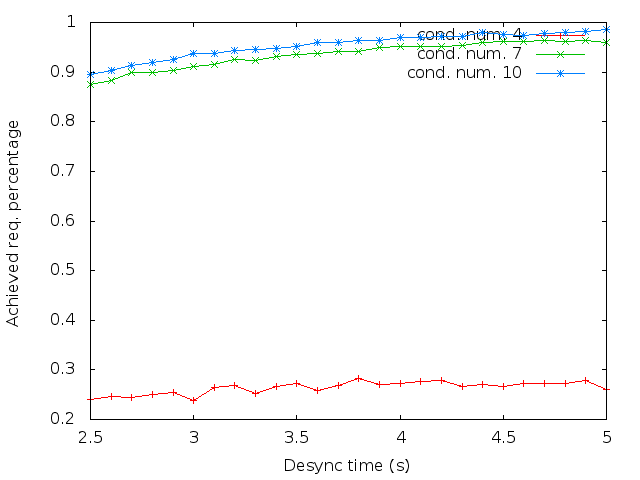
\includegraphics[width=0.4\textwidth]{octagonsimulation/achievedlocreq3preempt1drop0speed2.png}
    \label{fig:octagonsimulation/achievedlocreq3preempt1drop0speed2}}
    \hfill
    \subfloat[4 risposte]{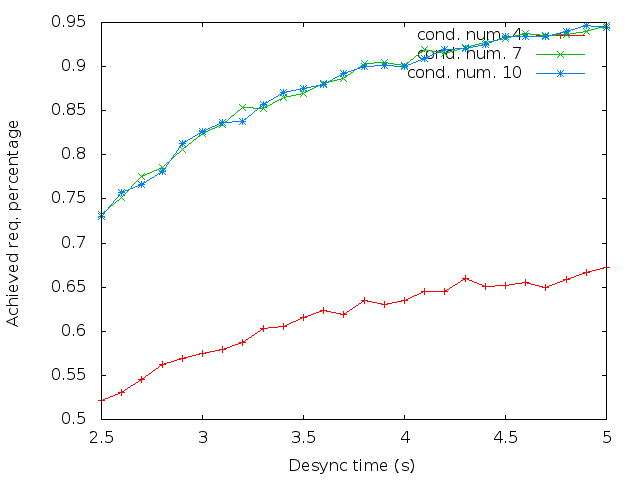
\includegraphics[width=0.4\textwidth]{octagonsimulation/achievedlocreq4preempt1drop1speed2.png}
    \label{fig:octagonsimulation/achievedlocreq4preempt1drop1speed2}}
    \caption{Localizzazioni riuscite}
\end{figure}

\begin{figure}[H]
    \centering
    \subfloat[3 risposte]{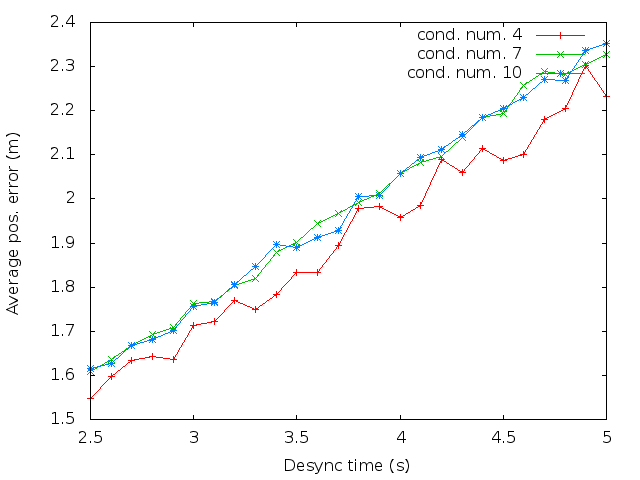
\includegraphics[width=0.4\textwidth]{octagonsimulation/avposerrorreq3preempt1drop0speed2.png}
    \label{fig:octagonsimulation/avposerrorreq3preempt1drop0speed2}}
    \hfill
    \subfloat[4 risposte]{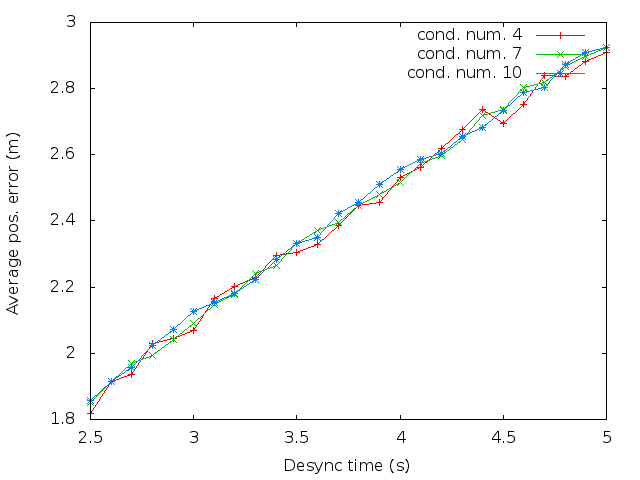
\includegraphics[width=0.4\textwidth]{octagonsimulation/avposerrorreq4preempt1drop1speed2.png}
    \label{fig:octagonsimulation/avposerrorreq4preempt1drop1speed2}}
    \caption{Errore medio}
\end{figure}

\begin{figure}[H]
    \centering
    \subfloat[3 risposte]{\includegraphics[width=0.4\textwidth]{octagonsimulation/maxposerrorreq3preempt1drop0speed2.png}
    \label{fig:octagonsimulation/maxposerrorreq3preempt1drop0speed2}}
    \hfill
    \subfloat[4 risposte]{\includegraphics[width=0.4\textwidth]{octagonsimulation/maxposerrorreq4preempt1drop1speed2.png}
    \label{fig:octagonsimulation/maxposerrorreq4preempt1drop1speed2}}
    \caption{Errore massimo}
\end{figure}
I risultati ottenuti sono molto simili a quelli per la topologia a 6 nodi (\ref{fig:hexagonsimulation/achievedlocreq3preempt1drop0speed2}, \ref{fig:hexagonsimulation/avposerrorreq3preempt1drop0speed2}, \ref{fig:hexagonsimulation/maxposerrorreq3preempt1drop0speed2}).


\section{Conclusioni}
Per quanto riguarda la configurazione economicamente piu' facilmente approntabile (quella con 4 nodi fissi), abbiamo ottenuto dei risultati abbastanza incoraggianti. Con l'AUV fermo, la precisione garantita di circa 10 $cm$ rende il protocollo  affidabile per un utilizzo concreto, considerando che nelle prove sul campo l'errore ottenuto sara' sicuramente piu' alto ma non troppo distante da questo valore notevolmente contenuto.
Risulta essere non ottimale, invece, la percentuale di localizzazioni andate a buon fine (nelle simulazioni non si e' riuscito a superare il  70\%). Considerando, invece, l'AUV in movimento, possiamo ritenere una percentuale di posizionamenti riusciti al 80\% un ottimo risultato e, per questo valore, otteniamo un errore medio di 1.7 $m$ ed uno massimo di circa 4 $m$. Se pensiamo alla missione simulata dal veicolo, ovvero il "monitoraggio" di un area quadrata di circa 200 $m$ di lato, l'accuratezza della posizione calcolata e' abbastanza accetabile. In situazioni del genere e' anche possibile, oltre a correggere il posizionamento grazie all'introduzione di tecniche di dead reckoning, fare in modo di fermare il veicolo, con una certa cadenza, e calcolarne le coordinate da fermo in maniera precisa, per poi riprendere lo svolgimento della missione.
\newline
Ovviamente, incrementando nodi fissi si ottengono risultati piu' precisi, ma per la velocita' di 1 $\frac{m}{s}$ il miglioramento rispetto alla topologia a 4 nodi non e' forse tale da giustificare il deployment di un maggion numero di nodi.
Ad esempio, con 8 nodi potremmo ottenere la precisione di circa 1 $m$ con il 90\% di localizzazioni riuscite, ovvero miglioreremmo la precisione rispetto alla configurazione con la meta' dei nodi di solamente 70 $cm$ (la percentuale di successo del 10\%) raddoppiando il costo del network necessario.
Diverso e' il discorso se la missione di un veicolo mobile richiede che esso si sposti a velocita' piu' elevate. I risultati ottenuti simulando il movimento dell'AUV a 2 $\frac{m}{s}$ mostrano notevoli differenze rispetto al numero di nodi fissi impiegati nella rete.
Con la topologia a 4 nodi, il risultato migliore che otteniamo e' un errore medio sulla posizione di 2.8 $m$ (errore massimo di 8 $m$), con percentuale di localizzazione riuscite dell'80\% e valore del timer di desincronizzazione pari a 4.5 $s$.
Aggiungendo due nodi alla topologia, l'errore medio scende a 1.65 $m$ e quello massimo a 5.5 $m$. Inoltre, la percentuale di localizzazioni andate a buon fine sale oltre l'80\% (circa l'83\%), con un tempo di desincronizzazione dei nodi fissi pari a 2.5 $s$, due secondi in meno rispetto alla topologia a 4 nodi. Cio' rappresenta un enorme guadagno in termini di accuratezza e precisione, oltre al vantaggio dovuto al minor tempo necessario alla localizzazione dell'AUV.
Utilizzando la topologia ad 8 nodi si ottengono risultati simili all'utilizzo di 6 nodi, se non che' per gli stessi valori degli errori e del timer di desincronizzazione si ottiene una percentuale di posizionamenti riusciti pari a circa il 90\%.








